% !TEX encoding = UTF-8 Unicode

\documentclass[a4paper]{article}

\usepackage{color}
\usepackage{url}
\usepackage[utf8]{inputenc} % make weird characters work
\usepackage{graphicx}

\usepackage[english,serbian]{babel}

\usepackage[unicode]{hyperref}
\hypersetup{colorlinks,citecolor=green,filecolor=green,linkcolor=blue,urlcolor=blue}

\newtheorem{primer}{Primer}[section]

\begin{document}

\title{Generisanje test primera za programe u C-u korišćenjem Fuzz tehnike\\ \small{Seminarski rad u okviru kursa\\Metodologija stručnog i naučnog rada\\ Matematički fakultet}}

\author{Ana Đorđević, Mladen Lazić, Aleksandra Đurić\\ djordjevicana93@gmail.com, mladen.lazic93@hotmail.com, \\ aleksandradjuric@mail.ru}
\date{9.~april 2015.}
\maketitle

\abstract{
%tekst apstrakta
\tableofcontents

\newpage

\section{Uvod}
\label{sec:uvod}
% tekst uvoda

\section{Testiranje}
\label{sec:testiranje}

Testiranje predstavlja važan deo životnog ciklusa razvoja softvera. Testiranjem se lakše uočavaju greške i propusti nastali prilikom implementacije. Pored toga ono predstavlja i jedan od načina specifikacije problema. Zbog prednosti koje se dobijaju čestim i redovnim testiranjem najzastupljenije i trenutno najpopularnije metodologije razvoja promovišu paralelno pisanje testova i implementacije softvera. Ekstremno programiranje kao jedan od predstavnika agilnih metodologija posebno ističe razvoj vođen testovima i pisanje testova prihvatljivosti \cite{agilnirazvoj}.


\subsection{Vrste testiranja}
\label{subsec:vrste_testiranja}
 
\subsection{Fuzz testiranje}
\label{subsec:fuzz_testiranje}

% Uloga Fuzz testiranja može i iznad (da ne bude poseban podnaslov)
\subsubsection{Uloga}
\label{subsubsec:uloga_fuzz_testiranja} 

\subsubsection{Vrste}
\label{subsubsec:vrste_fuzz_testiranja}

\subsubsection{Prednosti}
\label{subsubsec:prednosti_fuzz_testiranja}

\section{Implementacija Fuzz testera za C programe}
\label{sec:implementacija_fuzz_testera}

Softver koji smo napravili predstavlja Fuzz tester za programe napisane u C-u. Proverava se njihova robusnost. Programski jezik u kome je implementiran tester je C++. Neophodno je da C program pored izvornog koda ima i Makefile pomoću kog se dobija izvršni kod. U cilju pojednostavljivanja primene testera napravljen je jednostavan korisnički interfejs korišćenjem Qt biblioteka. 

\subsection{Zahtevi}
\label{subsec:zahtevi_testera}

Prilikom izučavanja teme seminarskog rada i iz ličnog iskustva prilikom pisanja koda u C-u zaključili smo da se dosta vremena gubi na zadavanje ulaza kojim se posmatra dotadašnje stanje napisanog programa i ispituje njegova ispravnost. Automatizacija ovog koraka donosi veliku uštedu vremena. Uz to, ovako se najlakše uočavaju greške i propusti nastali zbog neadekvatnog rukovanja unetim vrednostima. Na ovaj način se dodatno simuliraju i greške koje korisnici programa napisanih u programskom jeziku C mogu zadati kao input. Ako ulaz ne zadaje korisnik već neki drugi program tada ispravnost ulaza zavisi od ispravnosti programa koji generise ulaz i provere su takođe neophodne.\\

Neophodno je obezbediti dovoljno veliku količinu test primera koji će omogućiti što obuhvatniju proveru ulaznih podataka. Ove provere se obavljaju u cilju praćenja ponašanja napisanog programa. Svaki od različitih vrsta podataka koji se unose zahteva testiranje kako regularnima vrednostima tako i onim koje bi mogle predstavljati problem ukoliko rukovanje podacima nije dovoljno dobro implementirano. Ovo sve zahteva detaljnu analizu specifičnosti svakog tipa podataka koji je podržan testovima.

\subsection{Rešenja}
\label{subsec:resenja_koje_nudi_tester}

Tester ima grupu fajlova koji pokrivaju najčešće vrste ulaza koje C programi očekuju kao input. Svaki fajl pokriva po jedan tip inputa. Potrebno je napraviti listu tipova podataka koje program koji se testira očekuje na ulazu. Neophodno je voditi računa o ispravnom redosledu. Tester na osnovu napravljene liste popunjava novu listu. Svaki element te liste se dobija slučajnim izborom vrednosti iz fajla za zahtevani tip. Nova lista sa konkretnim vrednostima predstavlja ulazne podatke za izvršni program koji se testira. \\

Podržani su osnovni tipovi podataka: int, float, double i char. U svakom fajlu su sadržane neke od regularnih vrednosti, vrednosti koje su kritične za pojedine tipove i neke od potpuno pogrešnih vrednosti. U kritične vrednosti spadaju minimalne i maksimalne vrednosti za taj tip. Potpuno pogrešne vrednosti su one koje nisu primenjive na dati tip. \\

Omogućena je i provera nizovima čiji su elementi osnovni tipovi podataka. Moguće je zadati maksimalan ili tačan broj elemenata. Izbor ovog broja se može prepustiti i slučajnom odabiru. Glavni razlog dodavanja ove mogućnosti je provera ispravnosti rada programa u zavisnosti od toga da li se koriste dinamički ili statički alocirani nizovi. \\

Naš fuzz tester ima i test primere koji pokrivaju grupe stringova koje su specifične i često se upotrebljavaju. Obuhvaćene su sekvence karaktera koje predstavljaju datum, vreme, email adrese, putanje do fajlova. Ovo je implementirano kao demonstracija provere podacima koji nisu osnovni tipovi. \\

Segment koda koji vrši odabir jednog test primera:
\begin{verbatim}
/* uzima se element po element vektora koji 
čuva tip ulaznih podataka u zadatom redosledu */
for(unsigned i = 0; i < testType.size(); i++)
{
    std::string choosed = testType.at(i);
    
    /* u zavisnosti od tipa podatka u fajl 
    temp.txt se upisuje vrednost koja se dobija 
    slučajnim izborom jednog od elemenata vektora */
    if(choosed.compare("int") == 0)
    {
        /* vektor int_test se popunjava podacima iz fajla
        int.txt u kome se cuvaju svi test primeri za int */
        if(int_test.empty())
            fill_vector("int"); 
                 
        int rand_int = rand() % int_test.size();
        temp << QString::fromStdString(int_test.at(rand_int));
        temp << " ";
    ...
\end{verbatim}

Vrednosti korišćenog test primera kao i exit\_status programa se čuvaju u obliku izveštaja koji se potrebi može sačuvati.

\subsection{Korisnički interfejs}
\label{subsec:korisnicki_interfejs_testera}

Korisnički interfejs je napravljen da bi se korisnicima omogućila lakša upotreba testera. Pokušali smo da ga napravimo što intuitivnije i jednostavnije. 
Sa leve strane se nalazi lista koja predstavlja tipove podataka koji se očekuju na ulazu u odgovarajućem redosledu. Sa desne strane su dugmići kojima se dodaju elementi u listu. Za nizove se nudi i izbor broja elemenata. Klikom na dugme učitaj program se otvara prozor kojim se bira Makefile C programa koji se testira. Korisnik zadaje koliko puta će se pokrenuti program. Na slici \ref{fig:interfejs} je prikazan izgled korisničkog interfejsa. \\

\begin{figure}[h!]
\begin{center}
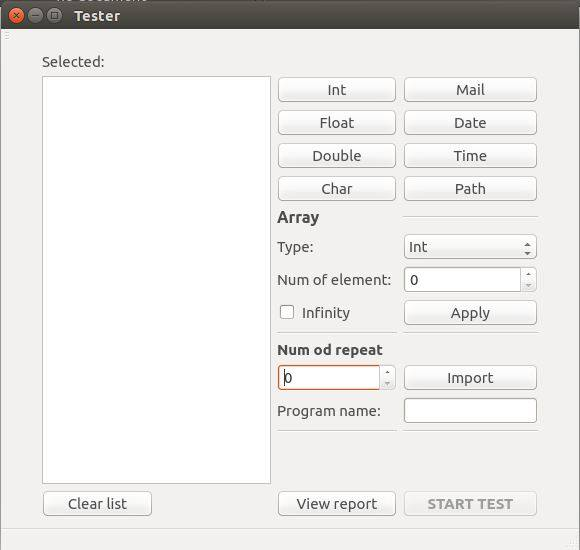
\includegraphics[scale=0.5]{korisnicki_interfejs.jpg}
\end{center}
\caption{Korisnički interfejs}
\label{fig:interfejs}
\end{figure}

Izveštaj rada se prikazuje u posebnoj formi u kojoj se pored informacija o vrednostima koje su korićene za svaki test primer čuva i informacija o tome kako se program završio u obliku exit\_statusa. Čuvanje ovog izveštaja na lokalnom disku je omogućeno klikom na dugme sačuvaj.

\section{Zaključak}
\label{sec:zakljucak}
%tekst zakljucka

\addcontentsline{toc}{section}{Literatura}
\appendix
\bibliography{seminarski} 
\bibliographystyle{plain}


\end{document}
